\subsection*{1D reads}

        The following histograms show the length distribution of 1D reads (both template and complement) for passes and fails.

        \begin{figure}[h!]
		\begin{subfigure}[b]{0.45\textwidth}
    			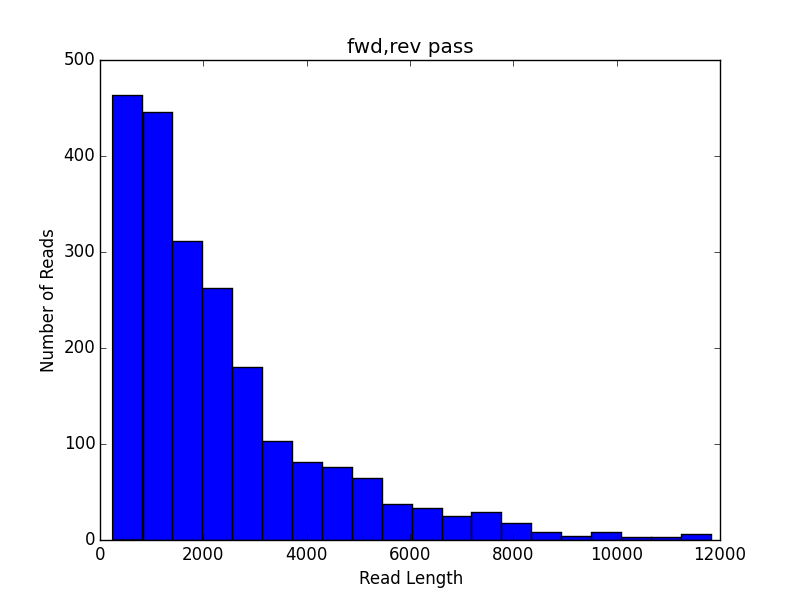
\includegraphics[width=3in]{1Dpasses}
    			\caption{Passed Reads}
  		\end{subfigure}
  		\begin{subfigure}[b]{0.45\textwidth}
    			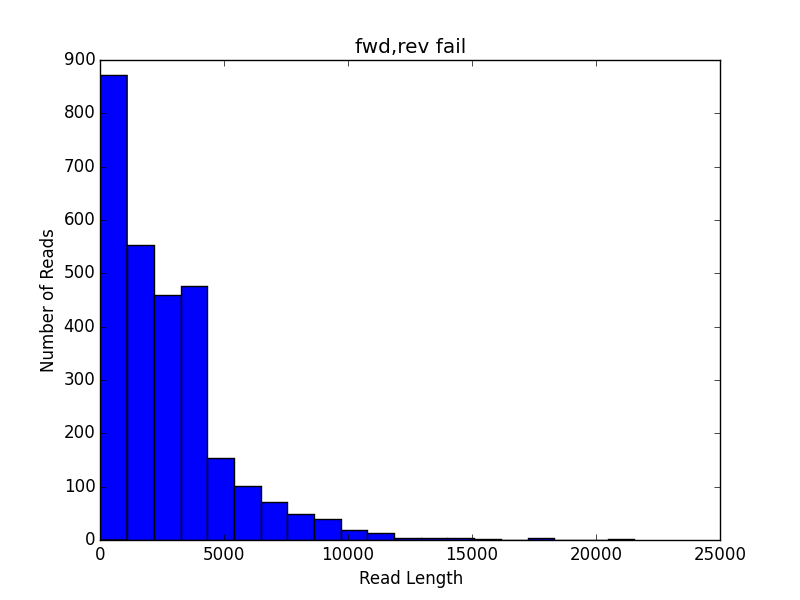
\includegraphics[width=3in]{1Dfailures}
    			\caption{Failed Reads}
  		\end{subfigure}
	\end{figure}
        

\subsection*{2D reads}

        The following histograms show the length distribution of 2D reads for passes and fails.

        \begin{figure}[h!]
		\begin{subfigure}[b]{0.45\textwidth}
    			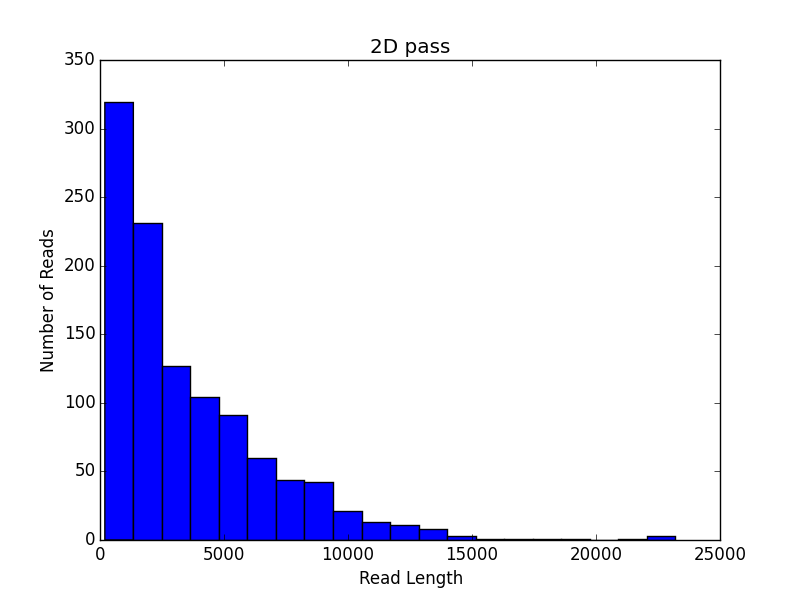
\includegraphics[width=3in]{2Dpasses}
    			\caption{Passed Reads}
  		\end{subfigure}
  		\begin{subfigure}[b]{0.45\textwidth}
    			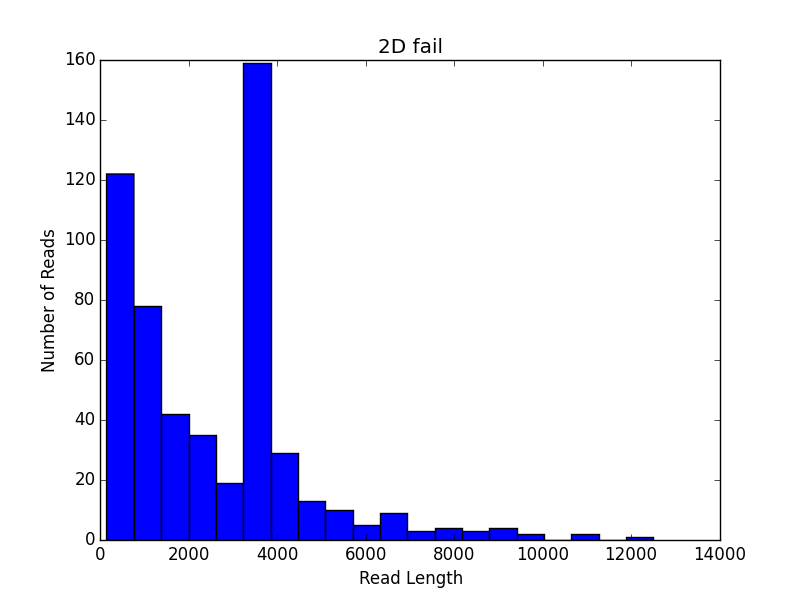
\includegraphics[width=3in]{2Dfailures}
    			\caption{Failed Reads}
  		\end{subfigure}
	\end{figure}

        
\subsection*{1D and 2D reads}

        The following histogramss show the cumulative length distribution of both 1D and 2D reads for passes and fails.

        \begin{figure}[h!]
		\begin{subfigure}[b]{0.45\textwidth}
    			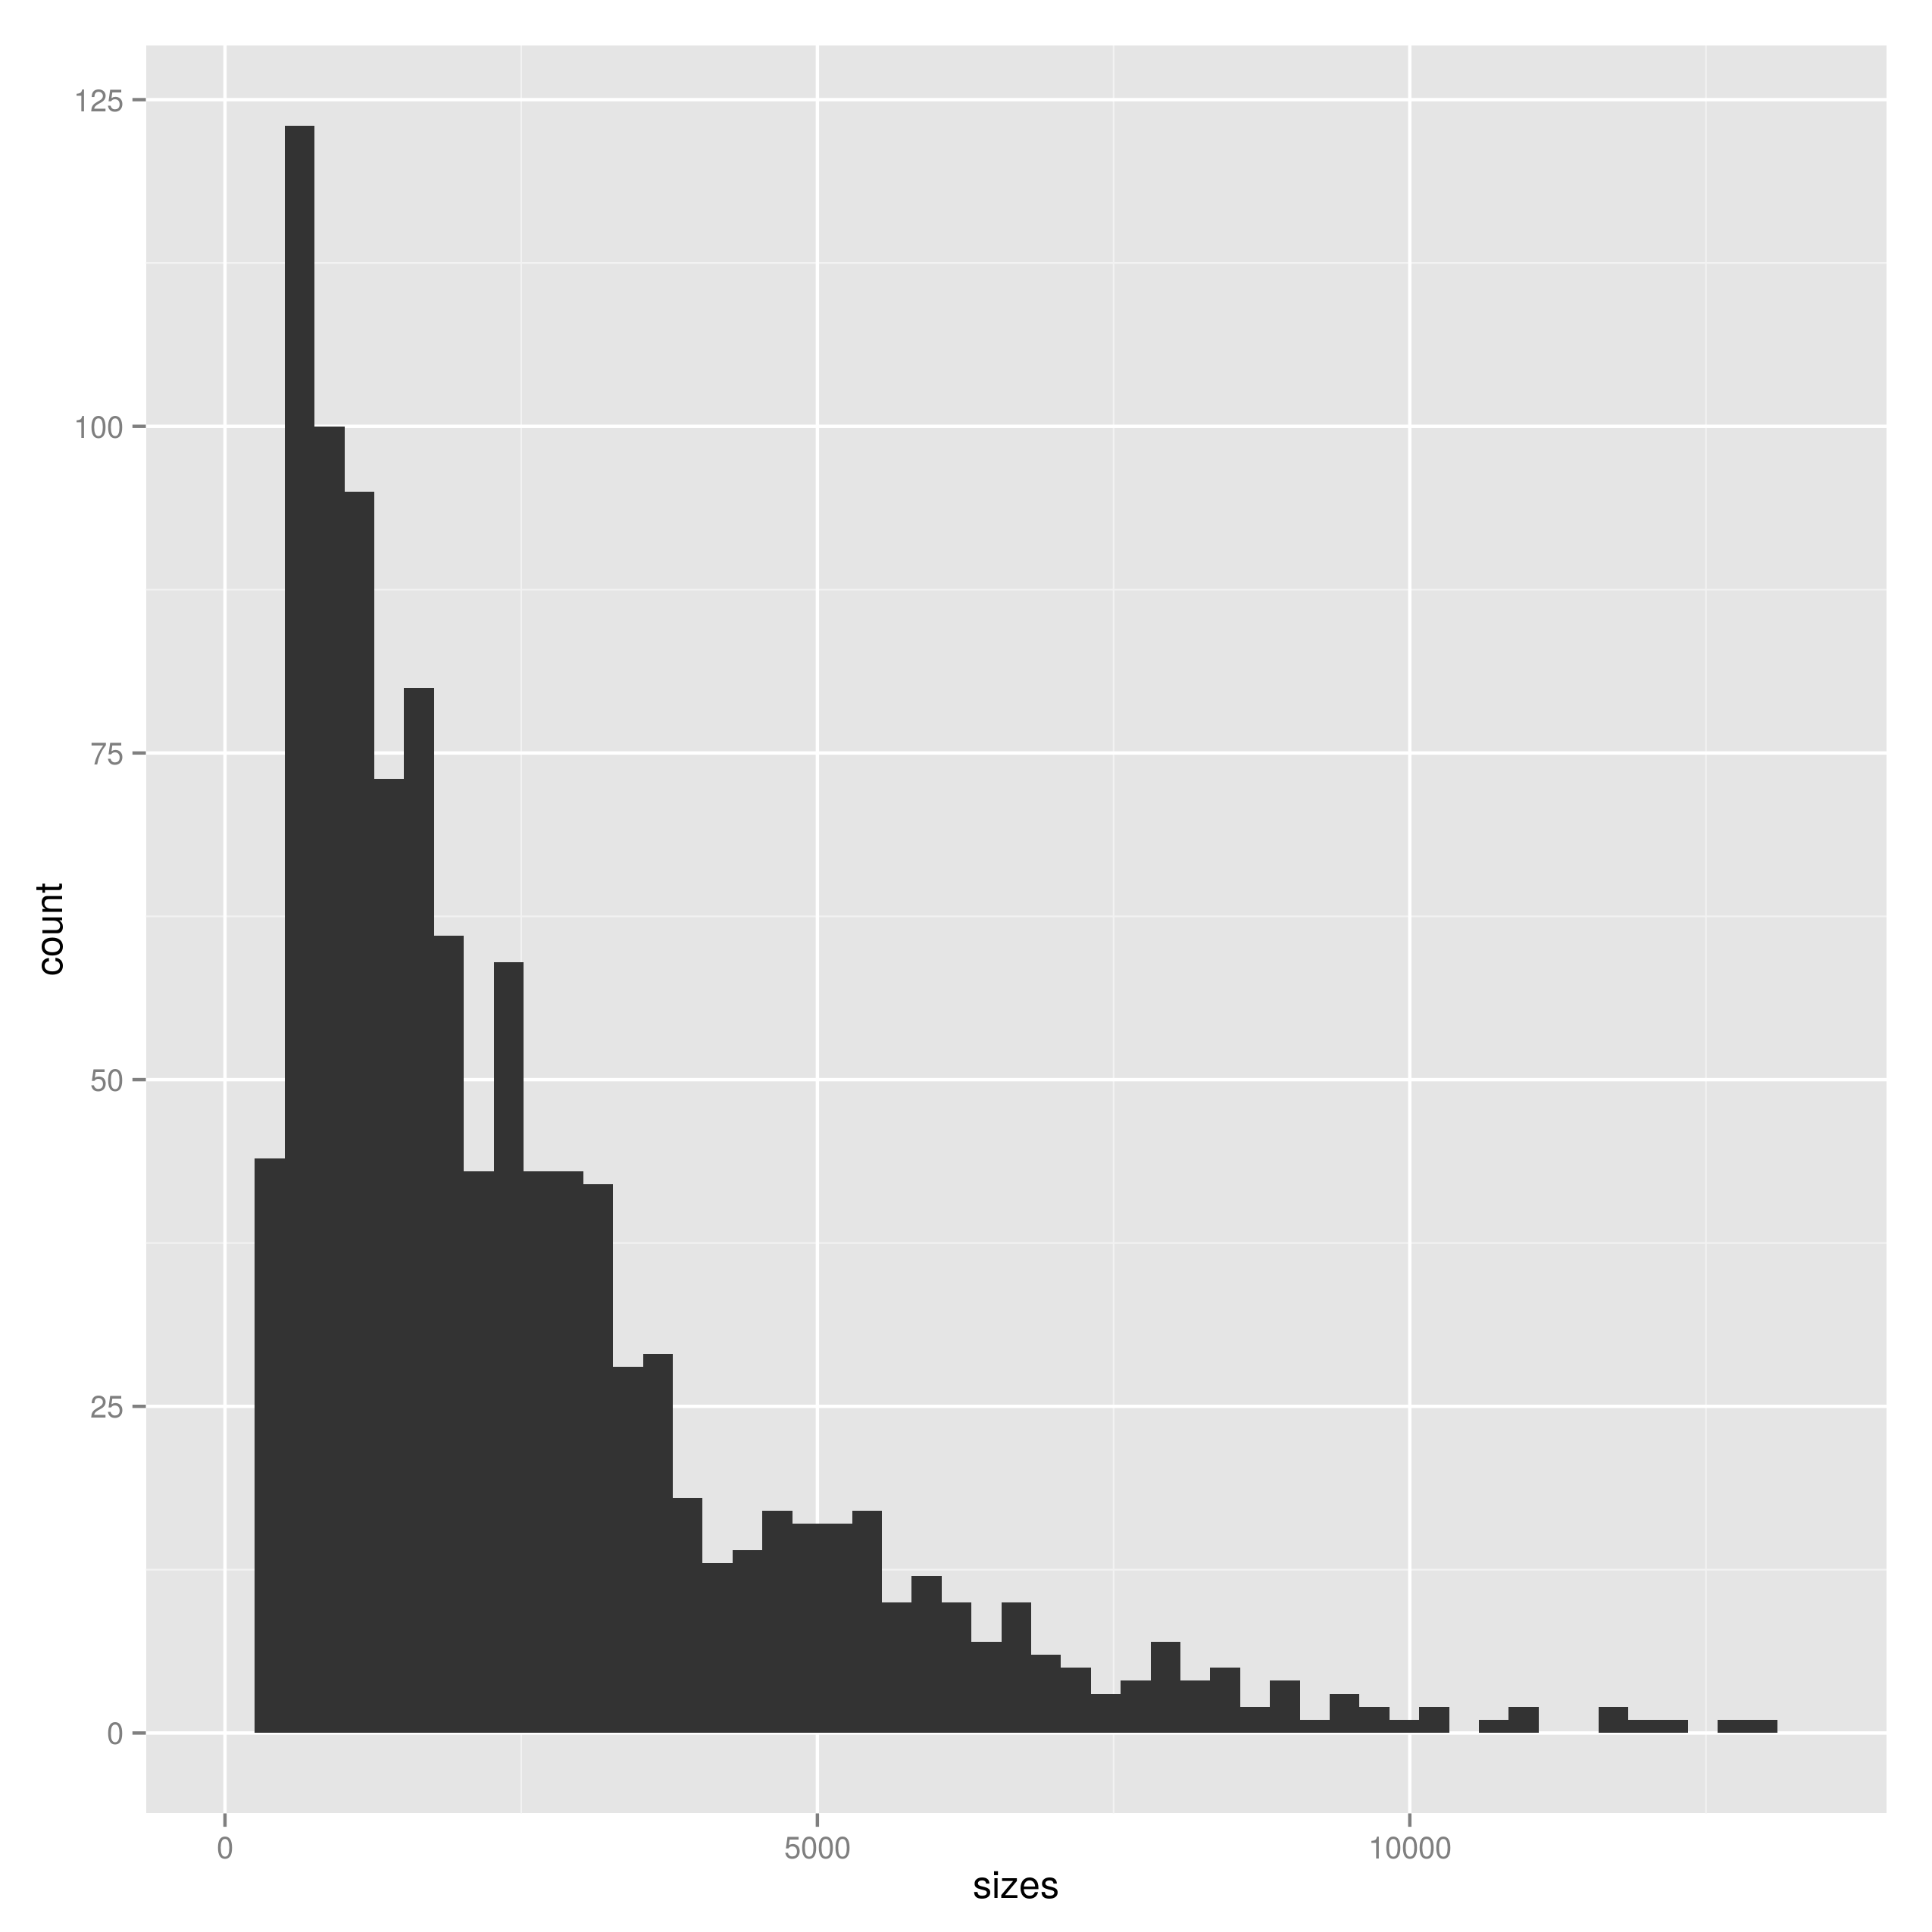
\includegraphics[width=3in]{histallpass}
    			\caption{Passed Reads}
  		\end{subfigure}
  		\begin{subfigure}[b]{0.45\textwidth}
    			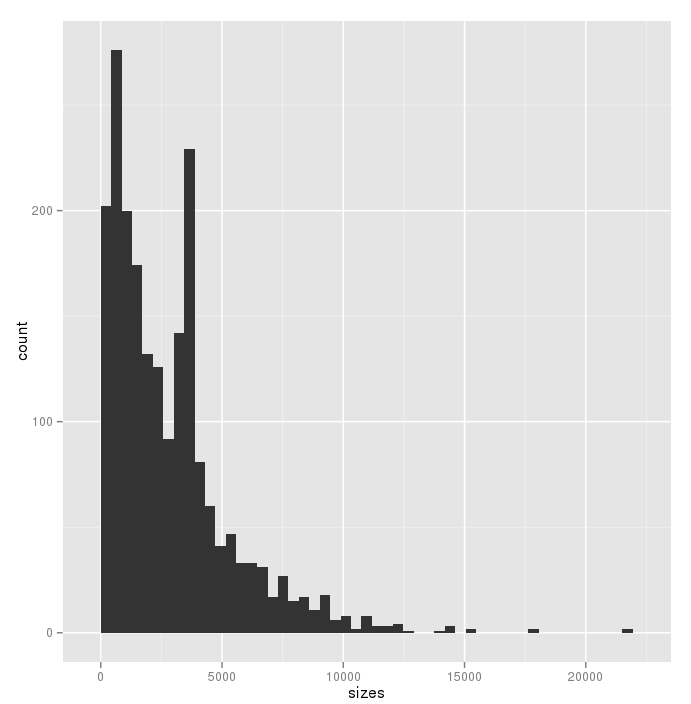
\includegraphics[width=3in]{histallfail}
    			\caption{Failed Reads}
  		\end{subfigure}
	\end{figure}
